\paragraph {Apple MVC}
Классическим архитектурным паттером при разработке для платформы iOS является \gls{mvc}. Шаблон присваивает объектам в приложении одну из трех ролей: модель, представление или контроллер. Шаблон определяет не только роли объектов в приложении, но и способ взаимодействия объектов друг с другом. Каждый из трех типов объектов отделен от других абстрактными границами и связывается с объектами других типов через эти границы. Набор объектов определенного типа \gls{mvc} в приложении иногда называется слоем, например, слоем модели. \cite{apple:mvc} На рисунке \ref{sec:analysis:research:mobArch:apple-mvc:image:mvc} представлена связь между объектами паттерна \gls{mvc}.

\begin{figure}[h]
  \centering
    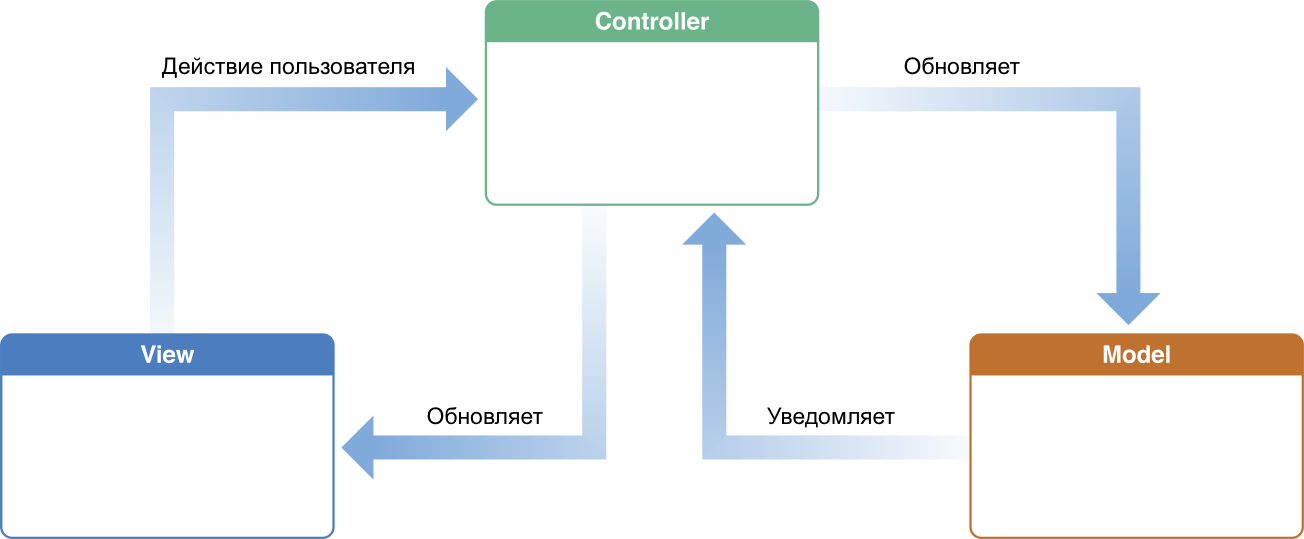
\includegraphics[width=1\textwidth]{inc/img/mvc.png}
  \caption{Связи между объектами MVC}
  \label{sec:analysis:research:mobArch:apple-mvc:image:mvc}
\end{figure}

\textbf{Объекты модели} инкапсулируют данные, специфические для приложения и описывают логику изменения этих данных. Для примера, объект модели может представлять персонажа в игре или контакт в книге контактов. Объекты модели могут иметь связь один ко многим или многие ко многим с остальными объектами модели, и поэтому иногда модельный уровень приложения представляет собой один или более объектных графов. В хорошей реализации паттерна объекты модели не должны иметь связи с объектами представления, изолируя данные от ошибок слоя презентации и действий пользователя: пользовательские действия в слое презентации, которые создают или модифицируют данные, влияют на модель при помощи промежуточного слоя котроллер и являются причиной создания или обновления объектов модели. Когда объект модели изменяется(например, новые данные были получены из сети), он уведомляет объект контроллера, который, в свою очередь, обновляет объект представления.

\textbf{Объектами представления} являются объекты, которые видит пользователь. Объекты данной группы умеют представлять себя графически на экране и реагировать на действия пользователя. Основной задачей объектов представления является вывести данные из модели приложения и позволить пользователю редактировать эти данные. Объекты представления часто обобщатся и используются между приложениями, хорошим примером такого переиспользования является \gls{uikit}. 

Объекты типа \textbf{котроллер} являются прослойкой между моделью и представлением, уведомляющих представление об изменениях в модели и наоборот. Объекты контроллера также могут выполнять настройку и координирование задач для приложения и управлять жизненными циклами других объектов. 